% Options for packages loaded elsewhere
\PassOptionsToPackage{unicode}{hyperref}
\PassOptionsToPackage{hyphens}{url}
%
\documentclass[
  a4paper,
]{scrbook}

\usepackage{amsmath,amssymb}
\usepackage{lmodern}
\usepackage{iftex}
\ifPDFTeX
  \usepackage[T1]{fontenc}
  \usepackage[utf8]{inputenc}
  \usepackage{textcomp} % provide euro and other symbols
\else % if luatex or xetex
  \usepackage{unicode-math}
  \defaultfontfeatures{Scale=MatchLowercase}
  \defaultfontfeatures[\rmfamily]{Ligatures=TeX,Scale=1}
  \setmainfont[]{Latin Modern Roman}
  \setsansfont[]{Latin Modern Roman}
\fi
% Use upquote if available, for straight quotes in verbatim environments
\IfFileExists{upquote.sty}{\usepackage{upquote}}{}
\IfFileExists{microtype.sty}{% use microtype if available
  \usepackage[]{microtype}
  \UseMicrotypeSet[protrusion]{basicmath} % disable protrusion for tt fonts
}{}
\makeatletter
\@ifundefined{KOMAClassName}{% if non-KOMA class
  \IfFileExists{parskip.sty}{%
    \usepackage{parskip}
  }{% else
    \setlength{\parindent}{0pt}
    \setlength{\parskip}{6pt plus 2pt minus 1pt}}
}{% if KOMA class
  \KOMAoptions{parskip=half}}
\makeatother
\usepackage{xcolor}
\setlength{\emergencystretch}{3em} % prevent overfull lines
\setcounter{secnumdepth}{5}
% Make \paragraph and \subparagraph free-standing
\ifx\paragraph\undefined\else
  \let\oldparagraph\paragraph
  \renewcommand{\paragraph}[1]{\oldparagraph{#1}\mbox{}}
\fi
\ifx\subparagraph\undefined\else
  \let\oldsubparagraph\subparagraph
  \renewcommand{\subparagraph}[1]{\oldsubparagraph{#1}\mbox{}}
\fi


\providecommand{\tightlist}{%
  \setlength{\itemsep}{0pt}\setlength{\parskip}{0pt}}\usepackage{longtable,booktabs,array}
\usepackage{calc} % for calculating minipage widths
% Correct order of tables after \paragraph or \subparagraph
\usepackage{etoolbox}
\makeatletter
\patchcmd\longtable{\par}{\if@noskipsec\mbox{}\fi\par}{}{}
\makeatother
% Allow footnotes in longtable head/foot
\IfFileExists{footnotehyper.sty}{\usepackage{footnotehyper}}{\usepackage{footnote}}
\makesavenoteenv{longtable}
\usepackage{graphicx}
\makeatletter
\def\maxwidth{\ifdim\Gin@nat@width>\linewidth\linewidth\else\Gin@nat@width\fi}
\def\maxheight{\ifdim\Gin@nat@height>\textheight\textheight\else\Gin@nat@height\fi}
\makeatother
% Scale images if necessary, so that they will not overflow the page
% margins by default, and it is still possible to overwrite the defaults
% using explicit options in \includegraphics[width, height, ...]{}
\setkeys{Gin}{width=\maxwidth,height=\maxheight,keepaspectratio}
% Set default figure placement to htbp
\makeatletter
\def\fps@figure{htbp}
\makeatother

\usepackage{titling}
\setlength{\droptitle}{-2cm}
\preauthor{
  \begin{center}
  \Large
  \vspace{10mm}
  by

  \vspace{20mm}
}
\postauthor{
  \end{center}
  \vfill
}

\predate{
  \begin{center}
  A thesis 
  submitted in fulfilment of the \\
  requirements of the degree of \\
  Doctor of Philosophy in Physics\\               % Degree
  School of Physical and Chemical Sciences\\          % Department
  Te Herenga Waka - Victoria University of Wellington\\                       % University 
  \vspace{5mm}
}
\postdate{
  \\
  
\includegraphics[width=3in,height=1.5in]{figures/VUW-logo.png}\\
  \end{center}
  }
\makeatletter
\makeatother
\makeatletter
\@ifpackageloaded{bookmark}{}{\usepackage{bookmark}}
\makeatother
\makeatletter
\@ifpackageloaded{caption}{}{\usepackage{caption}}
\AtBeginDocument{%
\ifdefined\contentsname
  \renewcommand*\contentsname{Table of contents}
\else
  \newcommand\contentsname{Table of contents}
\fi
\ifdefined\listfigurename
  \renewcommand*\listfigurename{List of Figures}
\else
  \newcommand\listfigurename{List of Figures}
\fi
\ifdefined\listtablename
  \renewcommand*\listtablename{List of Tables}
\else
  \newcommand\listtablename{List of Tables}
\fi
\ifdefined\figurename
  \renewcommand*\figurename{Figure}
\else
  \newcommand\figurename{Figure}
\fi
\ifdefined\tablename
  \renewcommand*\tablename{Table}
\else
  \newcommand\tablename{Table}
\fi
}
\@ifpackageloaded{float}{}{\usepackage{float}}
\floatstyle{ruled}
\@ifundefined{c@chapter}{\newfloat{codelisting}{h}{lop}}{\newfloat{codelisting}{h}{lop}[chapter]}
\floatname{codelisting}{Listing}
\newcommand*\listoflistings{\listof{codelisting}{List of Listings}}
\makeatother
\makeatletter
\@ifpackageloaded{caption}{}{\usepackage{caption}}
\@ifpackageloaded{subcaption}{}{\usepackage{subcaption}}
\makeatother
\makeatletter
\@ifpackageloaded{tcolorbox}{}{\usepackage[many]{tcolorbox}}
\makeatother
\makeatletter
\@ifundefined{shadecolor}{\definecolor{shadecolor}{rgb}{.97, .97, .97}}
\makeatother
\makeatletter
\makeatother
\ifLuaTeX
  \usepackage{selnolig}  % disable illegal ligatures
\fi
\usepackage[citestyle = ieee,urldate = iso8601]{biblatex}
\addbibresource{references.bib}
\IfFileExists{bookmark.sty}{\usepackage{bookmark}}{\usepackage{hyperref}}
\IfFileExists{xurl.sty}{\usepackage{xurl}}{} % add URL line breaks if available
\urlstyle{same} % disable monospaced font for URLs
\hypersetup{
  pdftitle={Volatile Organic Compound Detection Using Insect Odorant-Receptor Functionalised Field-Effect Transistors},
  pdfauthor={Eddyn Oswald Perkins Treacher},
  hidelinks,
  pdfcreator={LaTeX via pandoc}}

\title{Volatile Organic Compound Detection Using Insect Odorant-Receptor
Functionalised Field-Effect Transistors}
\author{Eddyn Oswald Perkins Treacher}
\date{Oct 2023}

\begin{document}
\frontmatter
\maketitle
\ifdefined\Shaded\renewenvironment{Shaded}{\begin{tcolorbox}[interior hidden, enhanced, borderline west={3pt}{0pt}{shadecolor}, breakable, sharp corners, frame hidden, boxrule=0pt]}{\end{tcolorbox}}\fi

\mainmatter
\bookmarksetup{startatroot}

\hypertarget{acknowledgements}{%
\chapter*{Acknowledgements}\label{acknowledgements}}
\addcontentsline{toc}{chapter}{Acknowledgements}

\markboth{Acknowledgements}{Acknowledgements}

\begin{verbatim}
69450
\end{verbatim}

Rifat, Alex - vapour sensor Erica Cassie - FET sensing setup Rob Keyzers
and Jennie Ramirez-Garcia - NMR spectra Patricia Hunt - Computational
chemistry

\bookmarksetup{startatroot}

\hypertarget{verifying-non-covalent-functionalisation-of-carbon-nanotubes-and-graphene}{%
\chapter{Verifying Non-Covalent Functionalisation of Carbon Nanotubes
and
Graphene}\label{verifying-non-covalent-functionalisation-of-carbon-nanotubes-and-graphene}}

\begin{verbatim}
159862
\end{verbatim}

In this chapter,

\hypertarget{non-covalent-functionalisation-and-linker-molecules}{%
\section{Non-Covalent Functionalisation and Linker
molecules}\label{non-covalent-functionalisation-and-linker-molecules}}

\hypertarget{pyrenebutanoic-acid-n-hydroxysuccinimide-ester-pbase}{%
\subsection{1-Pyrenebutanoic acid N-hydroxysuccinimide ester
(PBASE)}\label{pyrenebutanoic-acid-n-hydroxysuccinimide-ester-pbase}}

\begin{figure}

\begin{minipage}[t]{0.47\linewidth}

{\centering 

\raisebox{-\height}{

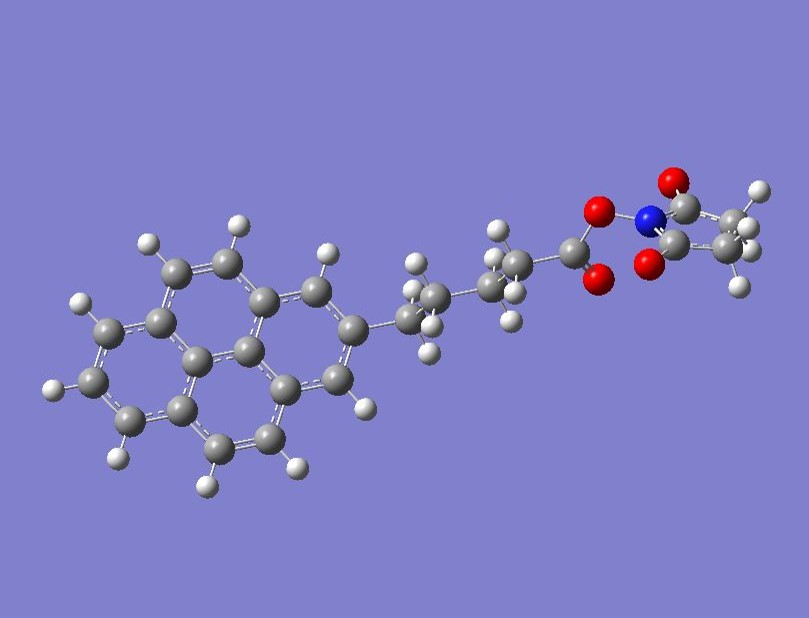
\includegraphics{./figures/ch6/pbase_stable_1.png}

}

}

\subcaption{\label{fig-pbase-stable-1}Hartree-Fock energy: -3427728.67
kJ/mol (9 s.f.)}
\end{minipage}%
%
\begin{minipage}[t]{0.05\linewidth}

{\centering 

~

}

\end{minipage}%
%
\begin{minipage}[t]{0.47\linewidth}

{\centering 

\raisebox{-\height}{

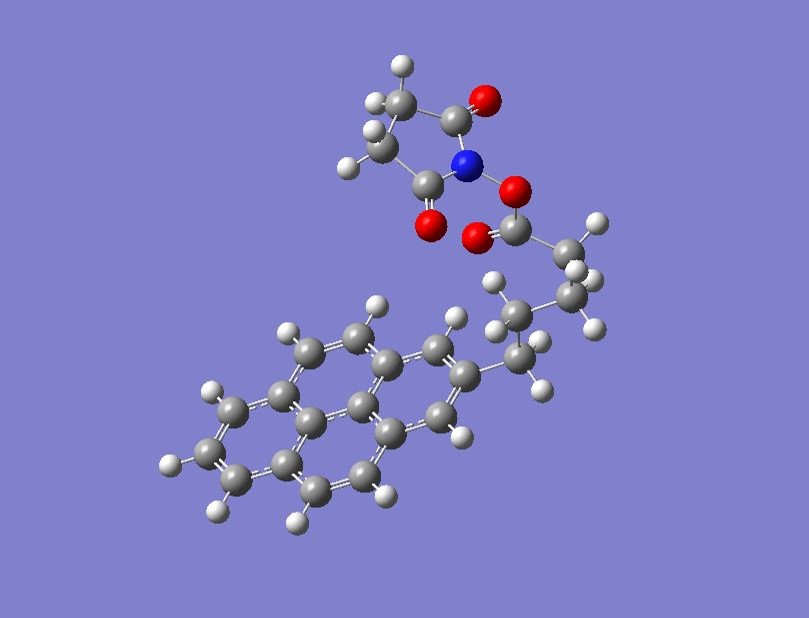
\includegraphics{./figures/ch6/pbase_stable_2.png}

}

}

\subcaption{\label{fig-pbase-stable-2}Hartree-Fock energy: -3427729.66
kJ/mol (9 s.f.)}
\end{minipage}%

\caption{\label{fig-pbase-structure}Two conformations of PBASE molecule
with geometry optimised via \emph{ab initio} calculation (computed using
Gaussian 16 \autocite{g16}). The difference between computed
Hartree-Fock energies is 1.0 kJ/mol, small enough that the existence of
both molecular conformations is physically possible.}

\end{figure}

1-Pyrenebutanoic acid N-hydroxysuccinimide ester (variously known
commercially and in the literature as 1-Pyrenebutyric acid
N-hydroxysuccinimide ester, PBASE, PBSE, PASE, Pyr-NHS, PyBASE, PANHS)
is a aromatic, bifunctional molecule commonly used for tethering
biomolecules to the carbon rings of graphene and carbon nanotubes. The
optimised molecular structure of PBASE is shown in
Figure~\ref{fig-pbase-structure}.

The non-covalent functionalisation of proteins onto a single-walled
carbon nanotube using PBASE was first reported by Chen \emph{et al.} in
2001 \autocite{Chen2001}. Two methods for protein functionalisation and
immobilisation were successfully used, with the only differences being
the solvent used to dissolve the PBASE powder (DMF, methanol) and the
final concentration of the resulting solutions (6 mM, 1 mM
respectively). The lower concentration may have been used for PBASE in
methanol as PBASE powder appears to dissolve poorly in methanol at
higher concentrations. Cella \emph{et al.}, Campos \emph{et al.}, Zheng
\emph{et al.} and Ohno \emph{et al.} all directly cite Chen \emph{et
al.} when discussing functionalisation with PBASE
\autocite{Cella2010,Campos2019,Zheng2016,Ohno2010}. Other groups using
PBASE for graphene or carbon nanotube functionalisation do not
explicitly reference Chen \emph{et al.} in their methodology, but it is
apparent they often draw on one of these two original methods. This
common ancestry becomes apparent from the high frequency of methods
detailing the use of 6 mM PBASE in DMF and 1 mM PBASE in methanol, as
seen in Table~\ref{tbl-pbase-functionalisation}.

However, despite this shared heritage, it is also apparent from
Table~\ref{tbl-pbase-functionalisation} that there is a large degree of
variation in the methods used for PBASE functionalisation. Various
electrical characterisation, microscopy and spectroscopy techniques have
been used to demonstrate successful functionalisation. However, there
has historically been little justification provided for the exact
parameters used in the procedure. As noted by Zhen \emph{et al.} and
Hinnemo \emph{et al.}, there is more generally a lack of systematic
research into formation of pyrene-derivative monolayers on graphene and
other carbon nanomaterials, despite the wide use of this chemistry in
the literature \autocite{Zhen2018,Hinnemo2017}.

\begin{figure}

\begin{minipage}[t]{\linewidth}

{\centering 

\raisebox{-\height}{

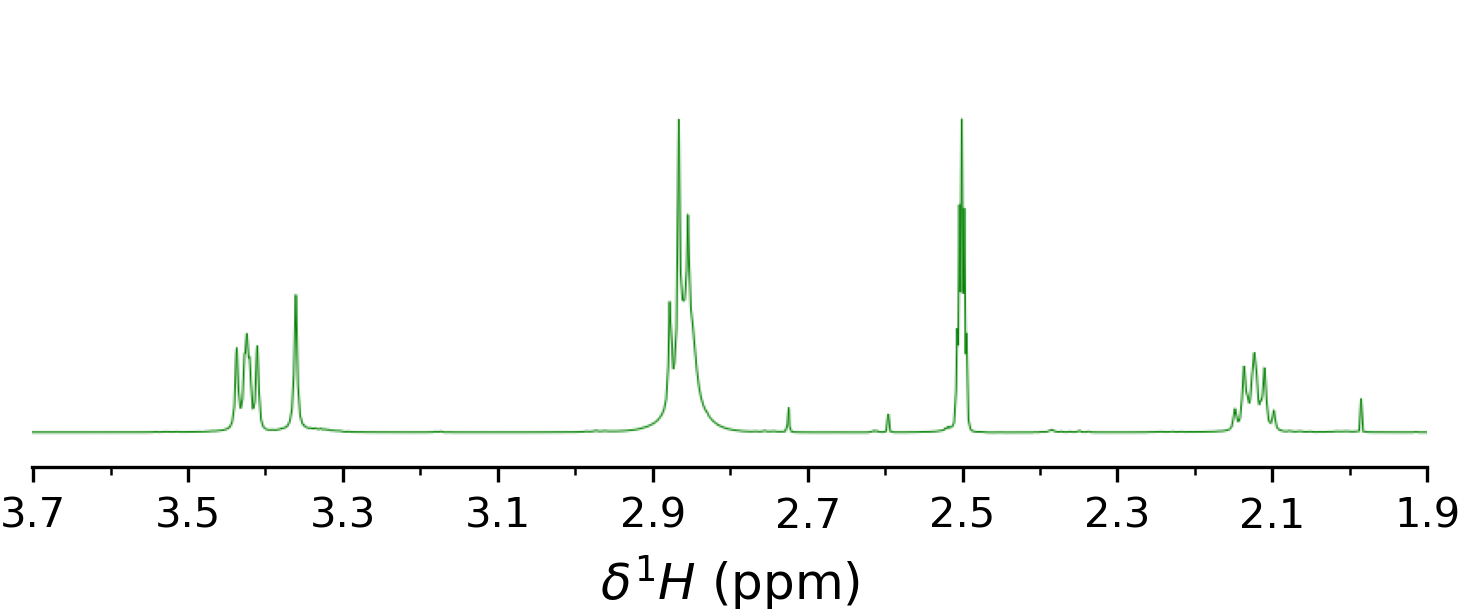
\includegraphics{./figures/ch6/modified_sigma_pbase_nmr.png}

}

}

\subcaption{\label{fig-sigma-nmr}}
\end{minipage}%
\newline
\begin{minipage}[t]{\linewidth}

{\centering 

\raisebox{-\height}{

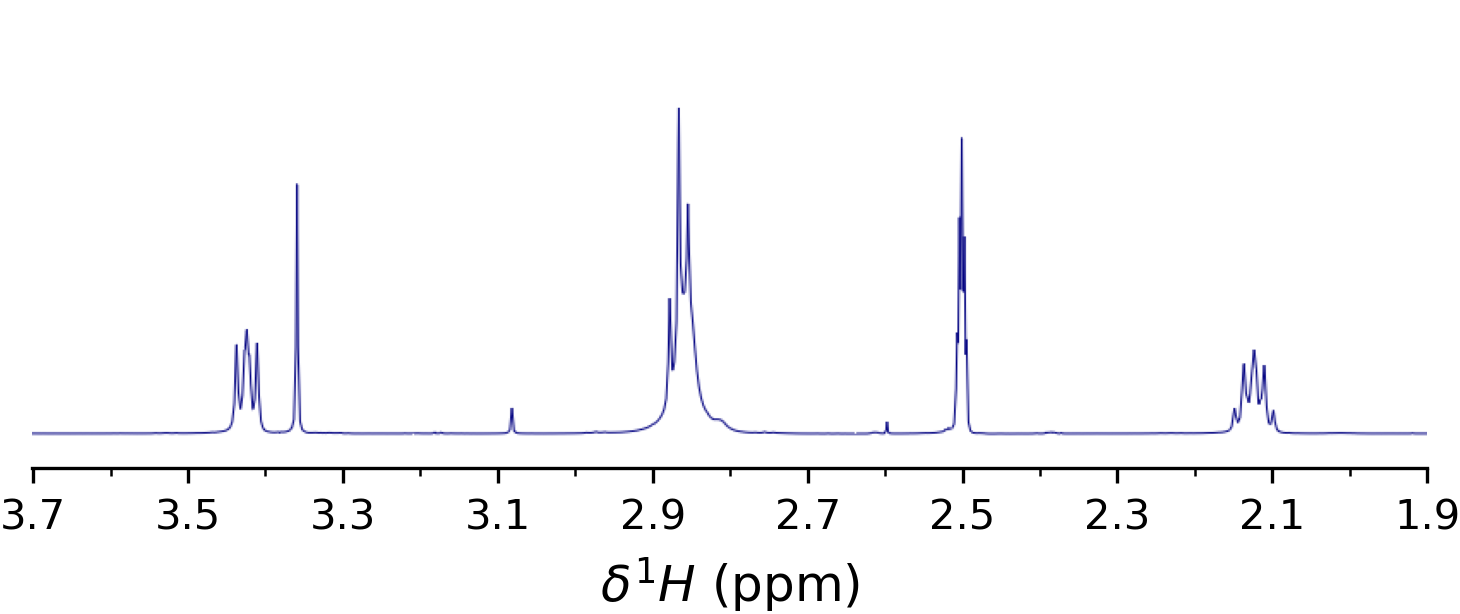
\includegraphics{./figures/ch6/modified_setareh_pbase_nmr.png}

}

}

\subcaption{\label{fig-setareh-nmr}}
\end{minipage}%
\newline
\begin{minipage}[t]{\linewidth}

{\centering 

\raisebox{-\height}{

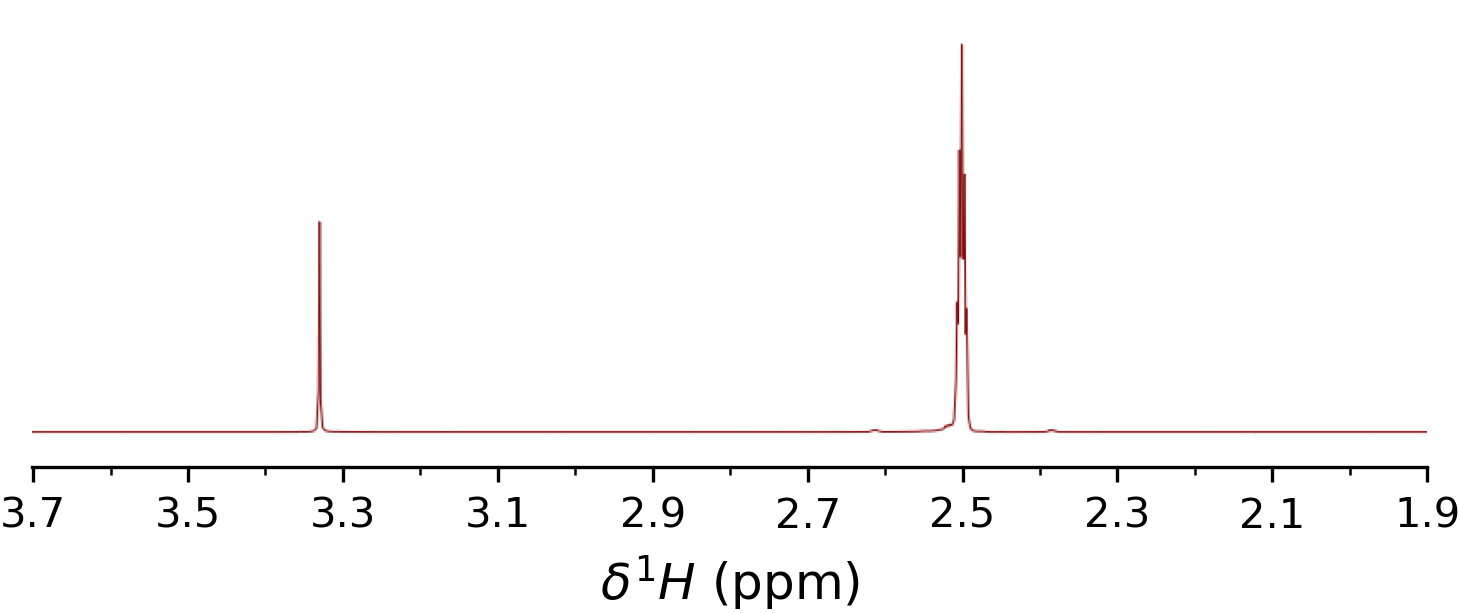
\includegraphics{./figures/ch6/modified_dmso_nmr.png}

}

}

\subcaption{\label{fig-dmso-nmr}}
\end{minipage}%

\caption{\label{fig-pbase-nmr}\(^{1}\)H Nuclear Magnetic Resonance (NMR)
spectra, performed with DMSO-d\(_6\) used as the NMR solvent. (a) and
(b) show NMR spectrum for commercially purchased PBASE, from
Sigma-Aldrich and Setareh Biotech respectively. (c) shows the blank
spectrum taken with only DMSO-d\(_6\) present .}

\end{figure}

We purchased PBASE from two suppliers, Sigma-Aldrich and Setareh
Biotech. Sigma recommends DMF and methanol as suitable solvents for
dissolving PBASE alongside chloroform and DMSO. Setareh Biotech
indicates methanol can be used for dissolving PBASE. The two suppliers
have conflicting information for suitable storage of PBASE, with Sigma
recommending room temperature storage while Setareh Biotech recommends
storage of \(-5\) to \(-30 ^\circ \text{C}\) and protection from light
and moisture. Figure~\ref{fig-pbase-nmr} compares the shapes of NMR
spectra of PBASE from each supplier dissolved in DMSO, alongside a blank
DMSO spectrum.

\newpage
\KOMAoptions{paper=landscape,pagesize}

\hypertarget{tbl-pbase-functionalisation}{}
\begin{longtable}[]{@{}llllrll@{}}
\caption{\label{tbl-pbase-functionalisation}Comparison of PBASE
functionalisation processes used for immobilisation of proteins and
aptamers onto liquid-gated CNTFET and graphene FET
sensors}\tabularnewline
\toprule()
Solvent & Channel & Conc. (mM) & Incubation type & Time (hr) & Rinse
steps & References \\
\midrule()
\endfirsthead
\toprule()
Solvent & Channel & Conc. (mM) & Incubation type & Time (hr) & Rinse
steps & References \\
\midrule()
\endhead
DMF & CNTs & 5 & Immersed & 1 & PBS & Maehashi \textit{et al.}
\cite{Maehashi2007} \\
& & 6 & Immersed & 1 & DMF, PBS & García-Aljaro \textit{et al.}
\cite{Garcia-Aljaro2010} \\
& & 6 & Immersed & 1 & DMF & Chen \textit{et al.} \cite{Chen2001} \\
& & 6 & Immersed & 1 & DMF & Cella \textit{et al.} \cite{Cella2010} \\
& & 6 & Immersed & 1 & DMF & Das \textit{et al.} \cite{Das2011} \\
& Graphene & - & - & 2 & DMF & Kwong Hong Tsang \textit{et al.}
\cite{KwongHongTsang2019} \\
& & - & - & 20 & - & Wiedman \textit{et al.} \cite{Wiedman2017} \\
& & 0.2 & Immersed & 20 & DMF, IPA, DI water & Gao \textit{et al.}
\cite{Gao2018} \\
& & 1 & 100 \(\mu\)L droplet & 6 & DMF, IPA, DI water & Nekrasov
\textit{et al.} \cite{Nekrasov2021} \\
& & 5 & Immersed & 1 & DMF, DI water & Hwang \textit{et al.}
\cite{Hwang2016} \\
& & 6 & 6 \(\mu\)L droplet & 2 & DMF, DI water & Nur Nasufiya
\textit{et al.} \cite{NurNasyifa2020} \\
& & 10 & 10 \(\mu\)L droplet & 2 & DMF, DI water & Campos
\textit{et al.} \cite{Campos2019} \\
& & 10 & Immersed & 2 & DMF, PBS & Kuscu \textit{et al.}
\cite{Kuscu2020} \\
& & 10 & Immersed & 1 & DMF & Xu \textit{et al.} \cite{Xu2017} \\
& & 10 & Immersed & 12 & DMF, ethanol, DI water & Khan \textit{et al.}
\cite{Khan2020} \\
2-Methoxyethanol & Graphene & 1 & Immersed & 1 & DI water & Ono
\textit{et al.} \cite{Ono2020} \\
Methanol & CNTs & 1 & Immersed & 1 & Methanol, DI water & Zheng
\textit{et al.} \cite{Zheng2016} \\
& & 1 & Immersed & 2 & Methanol & Kim \textit{et al.} \cite{Kim2009} \\
& Graphene & 5 & Immersed & 2 & - & Sethi \textit{et al.}
\cite{Sethi2020} \\
& & 5 & Immersed & 1 & Methanol, PBS & Ohno \textit{et al.}
\cite{Ohno2010} \\
DMSO & CNTs & 10 & - & 1 & DI water & Lopez \textit{et al.}
\cite{Lopez2015} \\
& & 10 & Immersed & 1 & PBS & Strack \textit{et al.}
\cite{Strack2013} \\
\bottomrule()
\end{longtable}

\newpage
\KOMAoptions{paper=portrait,pagesize}

\hypertarget{verifying-pyrene-attachment-to-cnt-network-and-graphene}{%
\section{Verifying Pyrene Attachment to CNT network and
graphene}\label{verifying-pyrene-attachment-to-cnt-network-and-graphene}}

\hypertarget{sec-photoresist-contamination}{%
\subsection{Photoresist
contamination}\label{sec-photoresist-contamination}}

\hypertarget{raman-spectroscopy}{%
\subsection{Raman Spectroscopy}\label{raman-spectroscopy}}

\hypertarget{pyrene-peg-fitc-fluorescence-microscopy}{%
\subsection{Pyrene-PEG-FITC fluorescence
microscopy}\label{pyrene-peg-fitc-fluorescence-microscopy}}

\hypertarget{plasma-clean-comparison}{%
\subsubsection*{Plasma clean comparison}\label{plasma-clean-comparison}}
\addcontentsline{toc}{subsubsection}{Plasma clean comparison}

\hypertarget{surfactant-comparison}{%
\subsubsection*{Surfactant comparison}\label{surfactant-comparison}}
\addcontentsline{toc}{subsubsection}{Surfactant comparison}

\hypertarget{pyrene-peg-electrical-characterisation}{%
\subsection{Pyrene-PEG electrical
characterisation}\label{pyrene-peg-electrical-characterisation}}

\appendix
\addcontentsline{toc}{part}{Appendices}

\hypertarget{sec-python}{%
\chapter{Python Code for Data Analysis}\label{sec-python}}

\hypertarget{code-repository}{%
\section{Code Repository}\label{code-repository}}

The code used for general analysis of field-effect transistor devices in
this thesis was written with Python 3.8.8. Contributors to the code used
include Erica Cassie, Erica Happe, Marissa Dierkes and Leo Browning. The
code is located on GitHub and the research group OneDrive, and is
available on request.

\hypertarget{sec-histogram-analysis}{%
\section{Atomic Force Microscope Histogram
Analysis}\label{sec-histogram-analysis}}

The purpose of this code is to analyse atomic force microscope (AFM)
images of carbon nanotube networks in .xyz format taken using an atomic
force microscope and processed in Gwyddion (see
\textbf{?@sec-afm-characterisation}). It was originally designed by
Erica Happe in Matlab, and adapted by Marissa Dierkes and myself for use
in Python.

\begin{equation}\protect\hypertarget{eq-lin-combo-gaussian}{}{
f(x) = k_1\exp{\Bigg(-\frac{{(x-m_1)}^{2}}{{2s_1}^{2}}\Bigg)} + k_2\exp{\Bigg(-\frac{{(x-m_2)}^{2}}{{2s_2}^{2}}\Bigg)} + ...
}\label{eq-lin-combo-gaussian}\end{equation}

The .xyz data is initially sorted into bins with 0.15 nm size. The bin
with the maximum number of counts is set at 0 nm, as this peak
represents the mean of the surface roughness of the bare silicon. The
parameters \(m_i\), \(s_i\), \(k_i\) (i = 1, 2, 3) are used with
objective function Equation~\ref{eq-lin-combo-gaussian} to overlay the
data with normal distributions. These fitting parameters represent the
mean (m), standard deviation (s) and amplitude (k) of each normal
distribution. We can make approximations of some of these fitting
parameters using the histogram data.

\(k_1\) is taken to be the maximum y-value of the data being fitted,
\(m_1\) is set to zero (used as a point of reference) and \(s_1\) is
taken as one-third of the difference between \(m_1\) and the x-value of
the first datapoint where the y-value is greater than 1\% of \(k_1\)
(approximating one standard deviation). We find the distribution given
by these values using Equation~\ref{eq-lin-combo-gaussian}, and subtract
it from the existing dataset.

Then, using the analysis technique outlined by Vobornik \emph{et al.}
\autocite{Vobornik2023} in Gwyddion, we manually find estimates for the
mean \(m_2\) and standard deviation \(s_2\) of the carbon nanotube
bundle distribution. We then take \(k_2\) to be the maximum y-value of
this modified dataset, and \(m_1\) to be the x-value of the maximum
y-value. We then set \(k_2\) so that the height of the resulting
distribution at one standard deviation matches the height of the .xyz
data histogram. We take this distribution, and subtract it from the
existing dataset.

The code also allows for discretely binning continuous data from fitted
normal distributions and examining the proportion of counts above or
below a particular height. 2.9 nm is roughly where 2 bundles with
average size 1.45 nm can start to be present, and is used as an estimate
of the boundary value between single-tube bundle diameters and
multi-tube bundle diameters.

\hypertarget{sec-field-effect-transistor-analysis}{%
\section{Field-Effect Transistor
Analysis}\label{sec-field-effect-transistor-analysis}}

The purpose of this code is to analyse electrical measurements taken of
field-effect transistor (FET) devices. Electrical measurements were
either taken from the Keysight 4156C Semiconductor Parameter Analyser,
National Instruments NI-PXIe or Keysight B1500A Semiconductor Device
Analyser as discussed in \textbf{?@sec-electrical-characterisation}; the
code is able to analyse data taken from all three measurement setups.
The main Python file in the code base consists of three related but
independent modules: the first analyses and plots sensing data from the
FET devices, the second analyses and plots transfer characteristics from
channels across a device, and the third compares individual channel
characteristics before and after a modification or after each of several
modifications. The code base also features a separate config file and
style sheet which govern the behaviour of the main code. The code base
was designed collaboratively by myself and Erica Cassie over GitHub
using the Sourcetree Git GUI.

The first of the three modules is for processing sensing datasets. This
module imports sensing measurements in .csv format and analyses them,
then outputs a plot of the raw data, alongside multiple plots which have
been modified in various ways. It can also fit exponential and linear
trendlines to regions of the sensing data, as well as find the signal
change per analyte addition, and returns spreadsheets containing the
results of these analyses. These spreadsheets include the standard
deviation for all included parameters. Modified plots include normalised
plots (type of normalisation can be set in config file), plots with
fitted curves, plots with the linear baseline drift removed, plots of
signal with analyte addition, ``despiked'' plots and ``filtered'' plots.
It is possible to add annotations to any of these plots using the config
file, and it is possible to produce a plot with a combination of these
modifications.

The scipy.optimize.curve\_fit module is used to fit linear and
exponential curves to regions of interest of the sensing data. Initial
parameters for the scipy.optimize.curve\_fit module are chosen by
approximating fitting parameters in a similar manner to the approach in
Section~\ref{sec-histogram-analysis}. For a linear fit \(mt + b\), the
parameters are simply set as \(m=1\) and \(b=0\). For an exponential fit
\(a\exp{(-t/\tau)} + c\), \(c\) is set as the final current measurement
of the region of interest and \(a\) is set as the initial current
measurement minus \(c\). Then, \(\tau\) is set as the time where current
has dropped to \(e^{-1}a + c\).

``Despiked'' plots have had spurious datapoints removed through the use
of an interquartile range rolling filter. The window size of the rolling
filter used was 40 datapoints, and datapoints in each window with a
z-score above \(\pm 3\) were removed from the plotted/processed data.
``Filtered'' plots had noise reduced using a moving median filter. The
moving median filter is more effective at removing noise than a simple
moving average, and has advantages over other filters (such as the
Savitzky-Golay filter) when removing noise from data with sharp edges,
as is the case for sensing data. Median filtering can also be used for
baseline drift compensation, though this approach was not used in this
thesis \autocite{Stone2011}. The moving median filter used had a window
of 40 datapoints.

Plots of signal with analyte addition were constructed from current data
after first removing baseline drift and applying a moving median filter.
A simple difference calculation between the mean of the filtered current
before an addition and the mean of the filtered current after the
addition was performed at each addition. These differences were then
normalised relative to the initial current. The signal with analyte
addition give reasonably consistent results regardless of whether
baseline drift was removed from the data, as shown in
Figure~\ref{fig-spaa-plot-comparison}. We can therefore be confident
that robust signal with analyte addition plots are robust even in the
presence of significant drift.

\begin{figure}

\begin{minipage}[t]{0.50\linewidth}

{\centering 

\raisebox{-\height}{

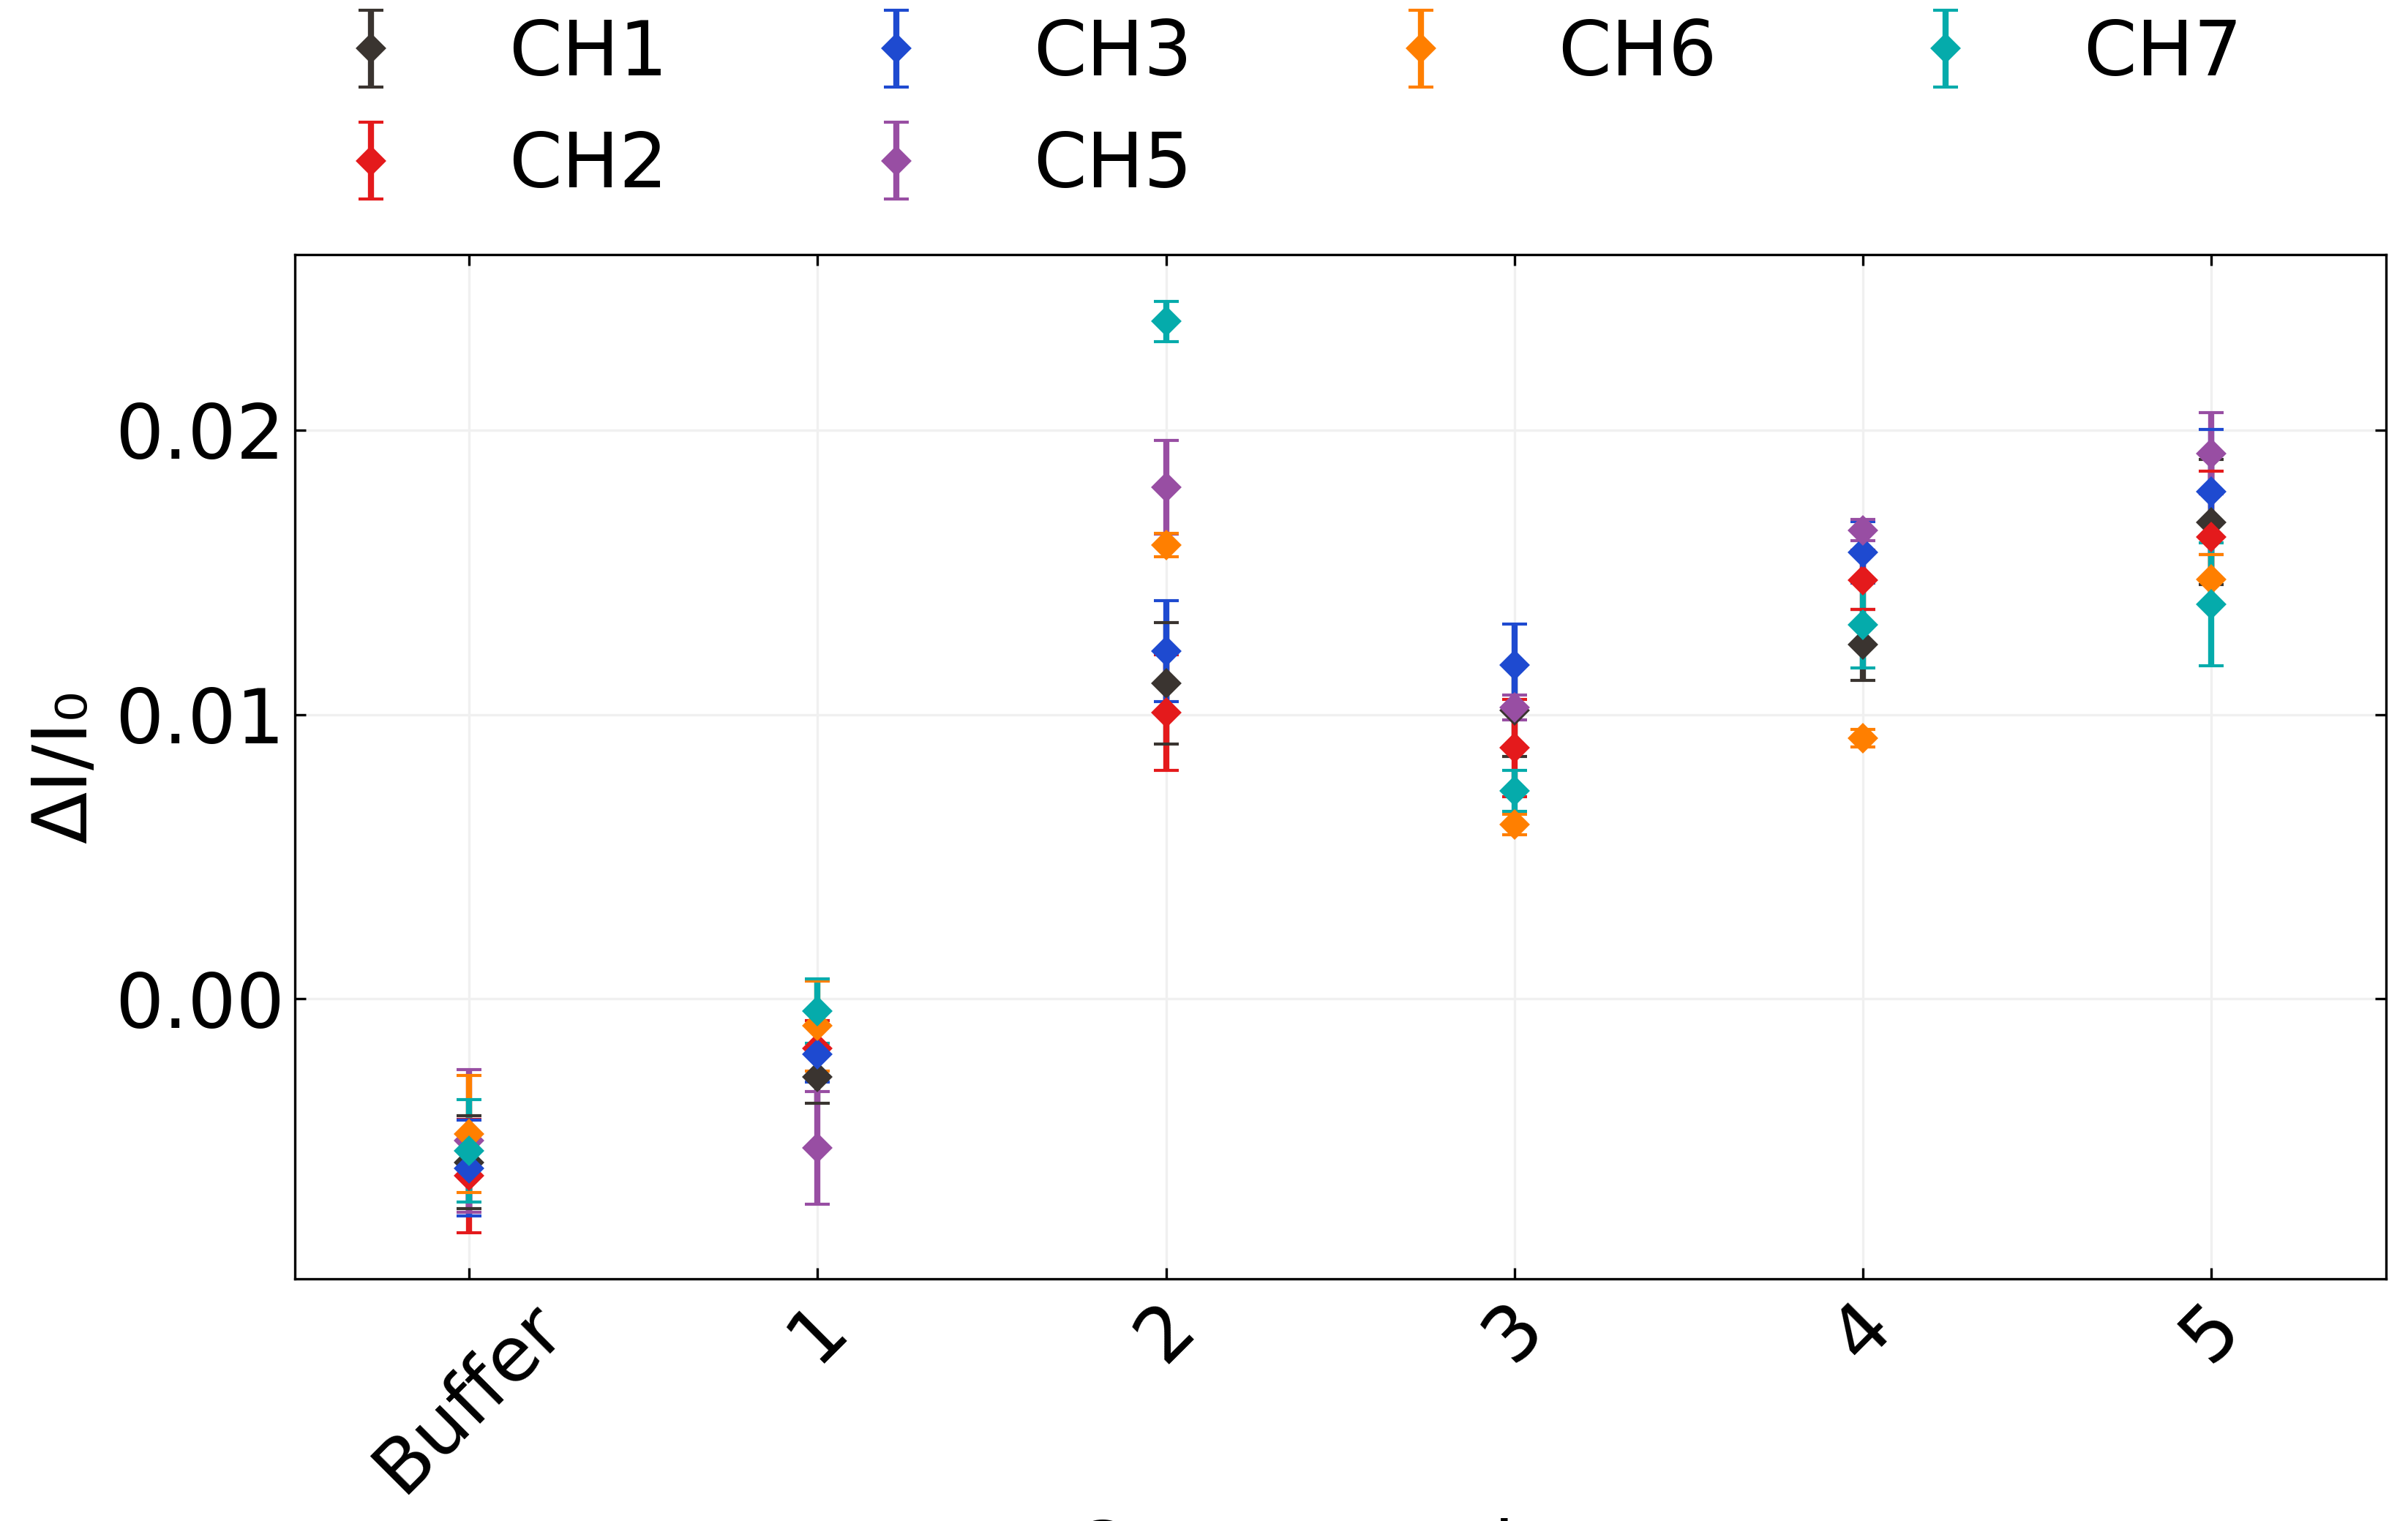
\includegraphics{./figures/app1/NTQ31C1_mean_simple_difference_before_and_after_step_filtered_concentrations.png}

}

}

\subcaption{\label{fig-spaa-no-detrend}}
\end{minipage}%
%
\begin{minipage}[t]{0.50\linewidth}

{\centering 

\raisebox{-\height}{

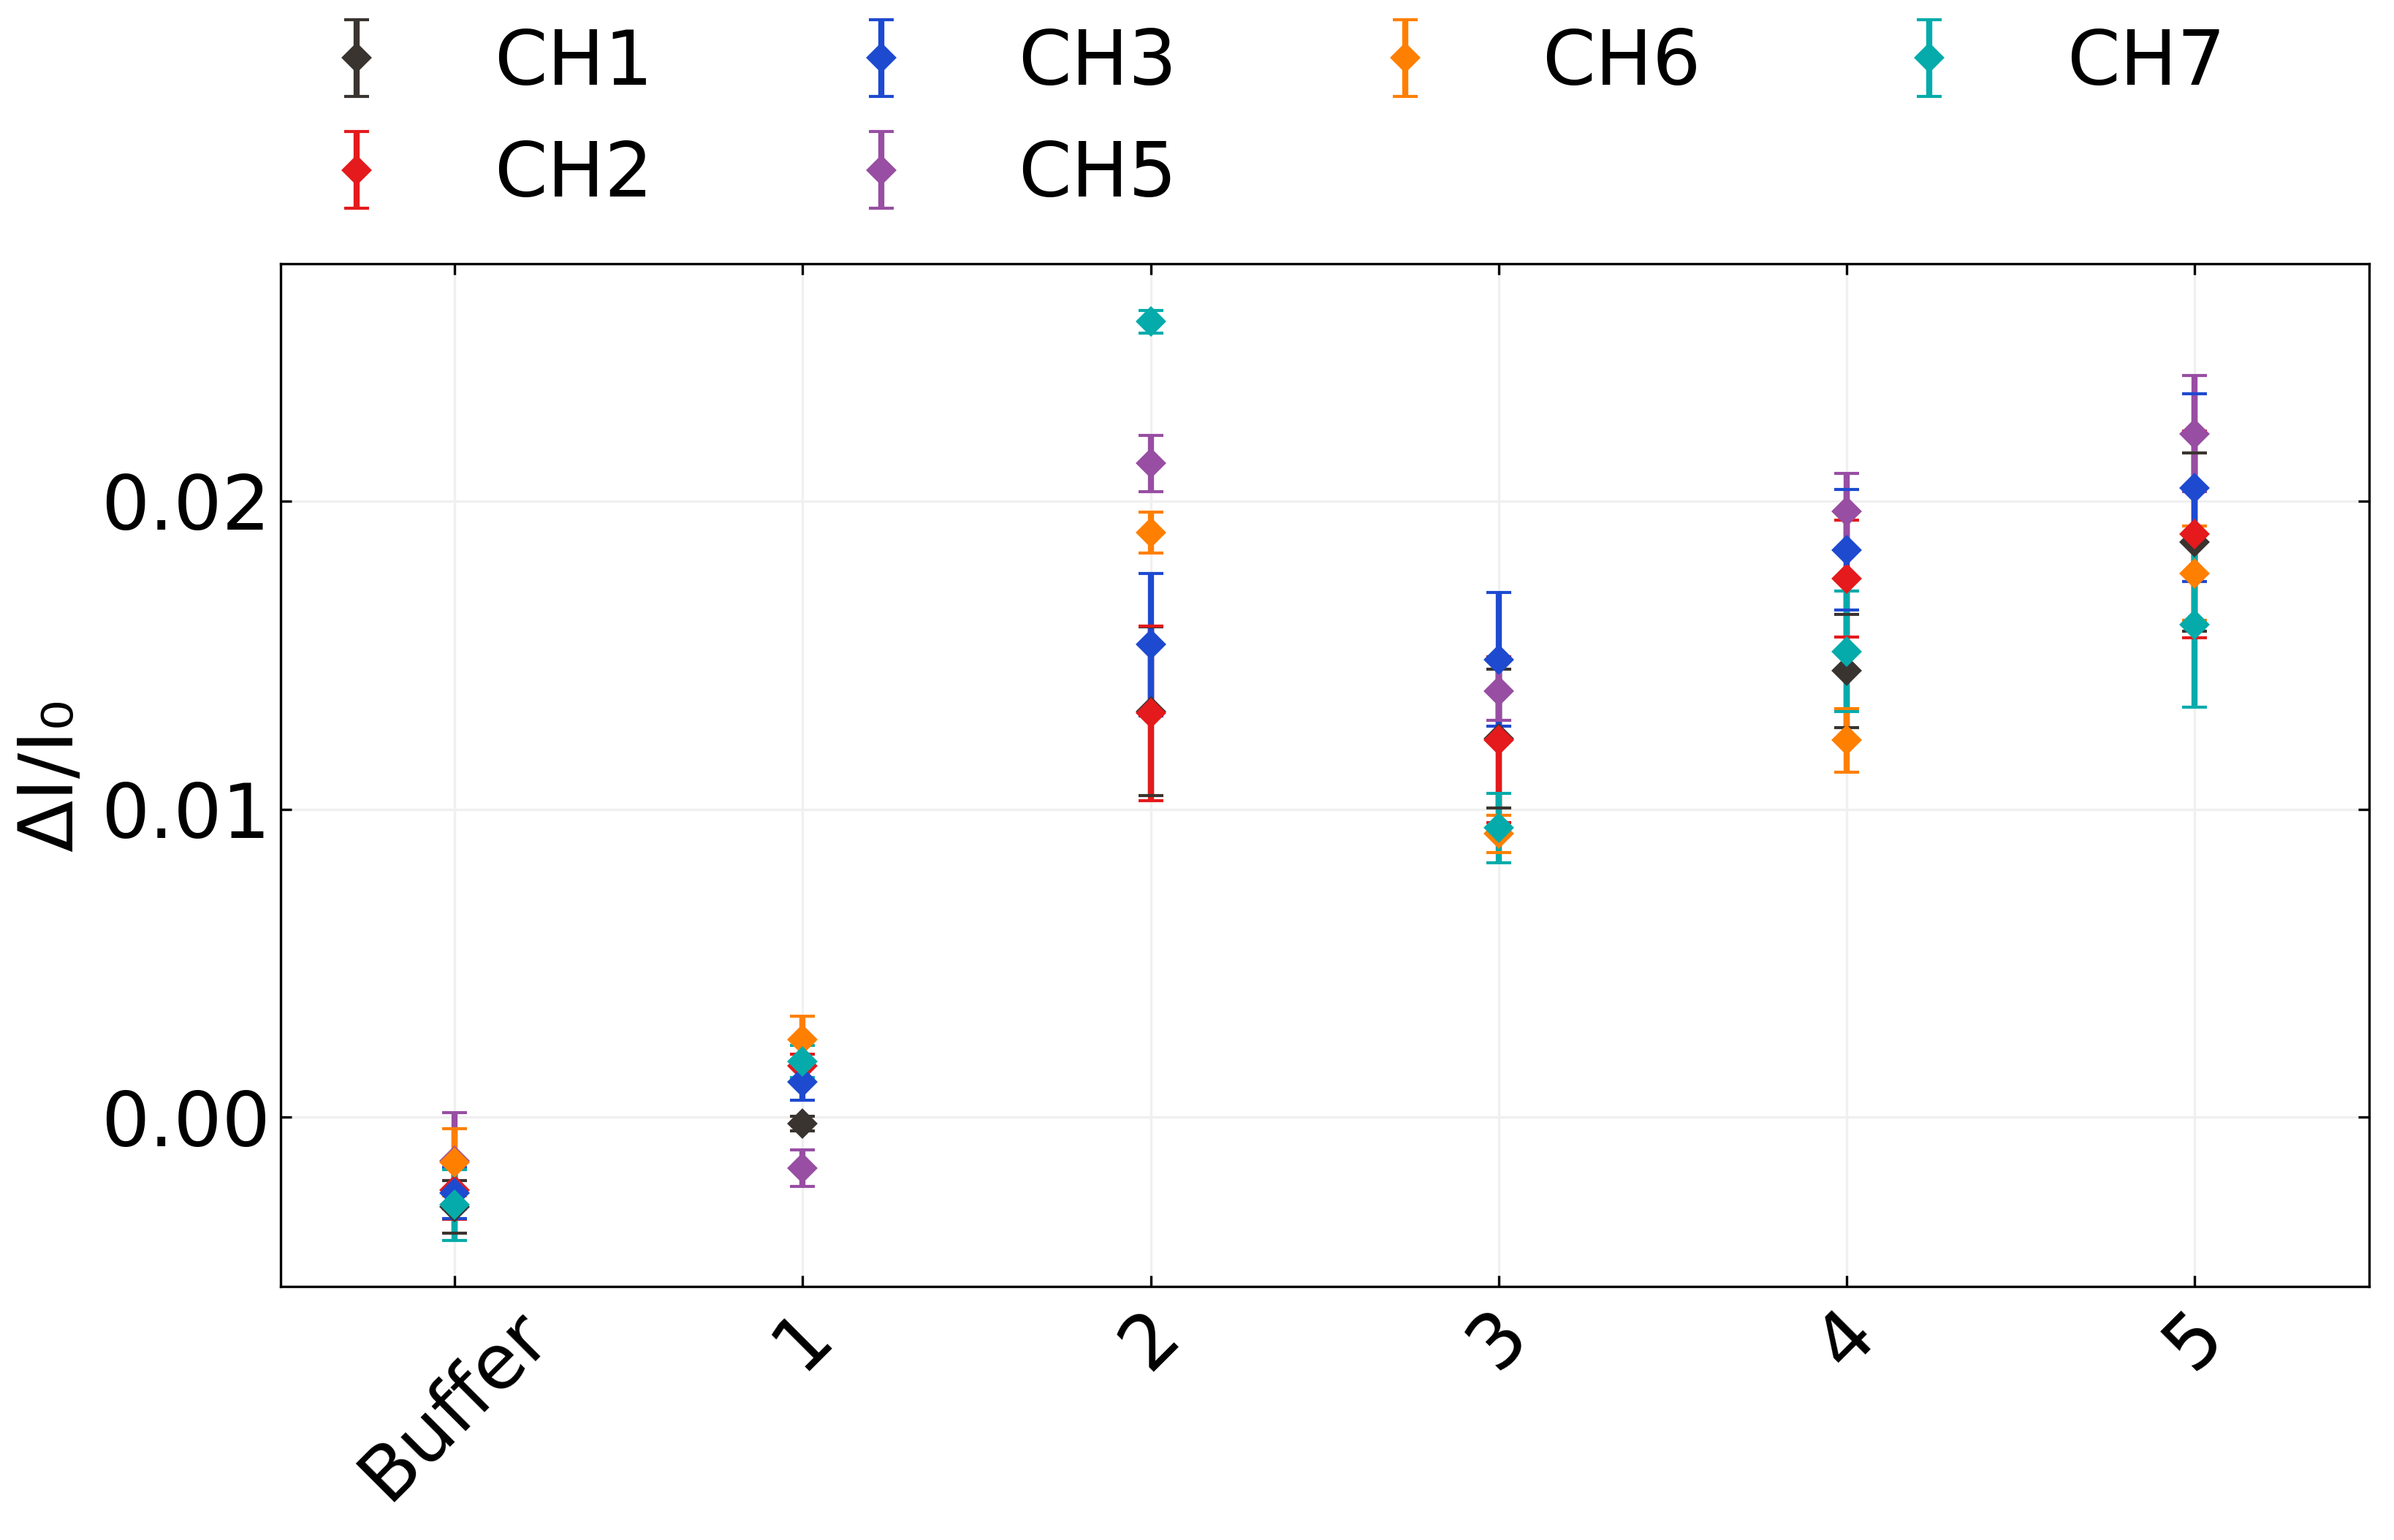
\includegraphics{./figures/app1/NTQ31C1_mean_simple_difference_before_and_after_step_filtered_concentrations_detrend.png}

}

}

\subcaption{\label{fig-spaa-detrend}}
\end{minipage}%

\caption{\label{fig-spaa-plot-comparison}A comparison of signal with
analyte addition plots taken from the same salt concentration sensing
dataset (the same dataset as used in \textbf{?@fig-salt-conc-sensing}).
In (a), a simple difference calculation performed on filtered data was
used, while in (b) the same calculation was performed on filtered data
with the baseline drift removed, the method used in the body of the
thesis.}

\end{figure}

The second module imports transfer measurements in .csv format and
creates combined and individual plots of the eight channels on a single
device. In combined plots, channels which are non-working, due to being
shorted or non-conducting, are removed via setting a maximum and minimum
possible on-current in the config file. Various parameters from the
transfer characteristics are saved as a spreadsheet along with standard
error. These parameters include on current, off current, subthreshold
slope and threshold voltage for the carbon nanotube devices, and on
current, off current and major Dirac point voltage for graphene devices.
The device type being analysed can be set in the config file.

The third module imports several transfer measurements in .csv format
and allows for comparison of the same channel before and after some
modification. It also calculates the shift in either threshold voltage
or major Dirac voltage of the device.

\hypertarget{vapour-delivery-system}{%
\chapter{Vapour Delivery System}\label{vapour-delivery-system}}

\hypertarget{technical-notes}{%
\section{Technical Notes}\label{technical-notes}}

Two LabView Virtual Instruments (VIs) were adapted from pre-existing VIs
for operating the mass flow controllers and monitoring vapour flow into
the device chamber, as well as monitoring temperature and humidity in
the vapour delivery system's manifold. These VIs were named ``\,'' A
third VI was developed in parallel which combined the first two Virtual
Instruments, alongside allowing the sequence of values to control the
mass flow controllers.

From Honours report: ``\,``\,'' Figure 12 gives the right side of the
front panel of the LabView VI sample with vapour.VI, which letsus preset
an autonomously-performed vapour sensing sequence. Each row in each
array module corresponds to a differennest step in this sequence. The
`howManySteps' module lets us set how many of these steps are performed.
The `Durations Array' module determines the length of time in seconds
each step is performed over. The `Carrier Flows Array' and `Dilution
Flows Array' modules let us set the carrier flow and dilution flow,
respectively, in standard cubic centimetres per minute (sccm) through
the gas rig at each step. The carrier flow pushes analyte vapour into
the vapour-sensing device chamber, while dilution flow is used to modify
the flow behaviour of the analyte vapour entering the chamber. The
vapour sensing sequence as depicted in Figure 12 was used for all vapour
sensing runs in this investigation. At the end of the sequence, the data
collected about the vapour sensing process was saved as an .lvm file.
``\,``\,''

\hypertarget{future-improvements}{%
\section{Future Improvements}\label{future-improvements}}


\backmatter
\printbibliography


\end{document}
